\documentclass[11pt,letterpaper]{article}
\pdfinfoomitdate=1\pdftrailerid{}\pdfsuppressptexinfo=15
\usepackage[T1]{fontenc}\usepackage[utf8]{inputenc}
\usepackage{lmodern,mathpazo,microtype}
\usepackage[margin=.88in,headheight=15pt]{geometry}
\usepackage{amsmath,amssymb,amsthm,mathtools}
\usepackage{graphicx,xcolor,booktabs,tabularx,array,enumitem,tikz}
\usetikzlibrary{arrows.meta,positioning,calc,fit,backgrounds}
\usepackage{titlesec,fancyhdr,needspace,placeins,listings,xurl}
\usepackage[numbers,sort&compress]{natbib}
\definecolor{ink}{HTML}{151224}\definecolor{violet}{HTML}{69469D}
\definecolor{gold}{HTML}{A47A29}\definecolor{mint}{HTML}{167569}
\definecolor{brightgold}{HTML}{E8BC69}\definecolor{brightmint}{HTML}{96DED2}
\definecolor{pale}{HTML}{F4F1FA}\definecolor{muted}{HTML}{615A70}
\usepackage[colorlinks=true,linkcolor=violet,citecolor=violet,urlcolor=mint,bookmarksnumbered]{hyperref}
\hypersetup{pdftitle={SUPER ALPHA: Inventing Economic Possibility},pdfauthor={Vincent Boucher},pdfsubject={Transformational Intelligence for creating valuable activities, sustaining advantage and compounding productive power},pdfkeywords={Super Alpha, Transformational Intelligence, economic possibility, invention, value capture, productive capacity}}
\urlstyle{same}\setlength{\emergencystretch}{3em}
\widowpenalty=10000\clubpenalty=10000\displaywidowpenalty=10000
\setlength{\parindent}{0pt}\setlength{\parskip}{5pt}\linespread{1.025}
\newcolumntype{Y}{>{\raggedright\arraybackslash}X}
\newcolumntype{P}[1]{>{\raggedright\arraybackslash}p{#1}}
\newcommand{\repo}{https://github.com/MontrealAI/AGI-Alpha-Invention-Flywheel-Lab}
\newcommand{\lead}[1]{\Needspace{5\baselineskip}\par\medskip\noindent{\large\sffamily\bfseries\color{violet}#1}\par\smallskip}
\newcommand{\thesis}[1]{\par\medskip{\sffamily\bfseries\large\color{violet}#1}\par\medskip}
\newcommand{\status}[1]{\textsf{\small #1}}
\newtheorem{proposition}{Proposition}\newtheorem{definition}{Definition}
\setlist{leftmargin=1.3em,itemsep=3pt,topsep=5pt}
\renewcommand{\arraystretch}{1.18}\setlength{\tabcolsep}{5pt}
\titleformat{\section}{\Large\sffamily\bfseries\color{ink}}{\color{violet}\thesection}{.6em}{}
\titleformat{\subsection}{\normalsize\sffamily\bfseries\color{ink}}{\thesubsection}{.6em}{}
\titlespacing*{\section}{0pt}{19pt}{8pt}\titlespacing*{\subsection}{0pt}{12pt}{5pt}
\pagestyle{fancy}\fancyhf{}\fancyhead[L]{\footnotesize\sffamily SUPER ALPHA}
\fancyhead[R]{\footnotesize\sffamily INVENTING ECONOMIC POSSIBILITY}
\fancyfoot[L]{\scriptsize\sffamily MONTREAL.AI / QUEBEC.AI}\fancyfoot[R]{\small\color{violet}\thepage}
\renewcommand{\headrulewidth}{.3pt}
\lstset{basicstyle=\footnotesize\ttfamily,columns=fullflexible,breaklines=true,keepspaces=true,showstringspaces=false}
\renewcommand{\topfraction}{.95}\renewcommand{\bottomfraction}{.9}\renewcommand{\textfraction}{.05}\renewcommand{\floatpagefraction}{.8}
\begin{document}
\hypersetup{pageanchor=false}
\begin{titlepage}\pagecolor{ink}\color{white}\thispagestyle{empty}

\begin{tikzpicture}[remember picture,overlay]
\fill[violet!35!ink] ([xshift=1cm,yshift=-2cm]current page.north east) circle (5.5cm);
\foreach \r in {4.2,4.8,5.4,6.0}{\draw[white,opacity=.045,line width=.7pt] ([xshift=1cm,yshift=-2cm]current page.north east) circle (\r cm);}
\draw[brightgold,line width=1.3pt] ([xshift=2.2cm,yshift=2.6cm]current page.south west)--([xshift=19.4cm,yshift=2.6cm]current page.south west);
\end{tikzpicture}
{\sffamily\small MONTREAL.AI / QUEBEC.AI\hfill\color{brightgold}RESEARCH EDITION 1.1}\par
\vspace{17mm}
{\sffamily\bfseries\fontsize{58}{60}\selectfont SUPER}\par
{\sffamily\bfseries\fontsize{69}{72}\selectfont ALPHA}\par\vspace{8mm}
{\sffamily\fontsize{24}{30}\selectfont Inventing Economic Possibility}\par\vspace{7mm}
{\sffamily\color{brightmint}\large TRANSFORMATIONAL INTELLIGENCE $\boldsymbol{\infty}$}\par
\vspace{10mm}
\begin{center}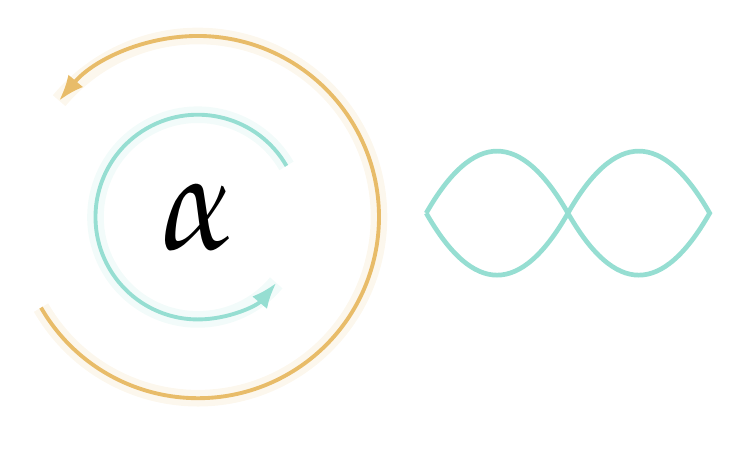
\begin{tikzpicture}[>=Latex]
\foreach \r/\a/\c in {1.3/30/brightmint,1.8/120/white,2.3/210/brightgold}{
\draw[\c,opacity=.12,line width=6pt] (\a:\r) arc[start angle=\a,end angle=\a+290,radius=\r];
\draw[\c,line width=1.4pt,->] (\a:\r) arc[start angle=\a,end angle=\a+290,radius=\r];}
\node[font=\fontsize{49}{50}\selectfont] at (0,0) {$\alpha$};
\draw[brightmint,line width=1.7pt] (2.9,.05) .. controls (3.5,1.1) and (4.1,1.1) .. (4.7,.05) .. controls (5.3,-1) and (5.9,-1) .. (6.5,.05) .. controls (5.9,1.1) and (5.3,1.1) .. (4.7,.05) .. controls (4.1,-1) and (3.5,-1) .. (2.9,.05);
\node[anchor=west,align=left,font=\sffamily\small,text=white!85] at (2.9,-1.45) {New possibilities.\\Renewable advantage.\\Greater productive power.};
\end{tikzpicture}\end{center}
\vfill
{\sffamily\bfseries\Large Invent what becomes possible.}\par\vspace{7mm}
{\large\bfseries Vincent Boucher}\par\smallskip
MONTREAL.AI\quad\textbullet\quad QUEBEC.AI\par
Montr\'eal, Qu\'ebec, Canada\par\medskip
{\small\color{white!75}3 November 2026\quad\textbullet\quad Version 1.1.0}
\vspace*{15mm}
\end{titlepage}\nopagecolor\color{ink}\hypersetup{pageanchor=true}

\thesis{An industry can be an invention.}
\begin{abstract}
The most consequential use of autonomous intelligence may be to construct valuable activities that existing complete methods cannot deliver economically. We call the resulting ambition \emph{SUPER ALPHA}: create an economic possibility, earn an extraordinary advantage in delivering it, and compound the resulting capabilities and retained surplus into further productive power. The object of invention is a complete arrangement comprising an outcome, production and verification means, voluntary participation, financing and operating policy. This paper integrates Transformational Intelligence with innovation economics and the AGI ALPHA research program. Its contribution is a joint account of scoped economic enablement, value capture under rival response, and four separately measurable compounding processes: commerce, capability inheritance, discovery improvement and physical production. An exact authored example shows how improved production and shared construction jointly enable profitable delivery when either change alone fails. A commercial price window specifies what must be invented; exact capital and qualification conditions determine whether its successor can be funded in time. We develop three industry hypotheses: scientific capability foundries, on-demand historical observation and adaptive industrial infrastructure. Their long-range consequence is a production network in which qualified instruments, useful energy and manufacturing capacity support increasingly powerful successors. The executable examples and reviewed public experiments retain their limits: strong conventional methods can tie or win, and commercial scale and physical expansion remain unestablished. The research objective is an enterprise that repeatedly constructs the conditions for its next consequential advantage.
\end{abstract}

\textbf{Blue Sky Super Alpha.} Inventing what the world could not economically do before, with an extraordinary advantage that creates immense value and compounds into vast, sustainable profit.

\textbf{The central question.} Which important activity is currently uneconomic because its means of production, evidence or cooperation are missing---and what construction could change that condition while leaving every participant better served?

\textbf{What this paper adds.} Earlier papers establish purpose-preserving reformulation, constructive instruments, viable market design and successor inheritance. SUPER ALPHA joins their consequences in a constructive sequence: quantify the economic change a valuable activity needs, construct its missing means, establish a viable share of its value under competition, and fund a qualified successor before its opportunity closes. Exact capital and timing conditions make that sequence testable; physical expansion supplies a further engineering requirement.

\textbf{Evidence at a glance.} New: an integrated research framework and reproducible, deliberately authored analytical examples. Source-reviewed: the pinned public experiment record. Proposed: new industries, better invention procedures and industrial expansion. No new customer revenue, native enterprise run, improved discovery result or physical deployment is reported here.

\clearpage
\section*{A map of the argument}
\addcontentsline{toc}{section}{A map of the argument}
\begin{tabularx}{\linewidth}{@{}P{3.0cm}YP{2.0cm}@{}}\toprule
Question & What the paper develops & Read\\\midrule
What could become possible? & Invent the complete productive arrangement; preserve the beneficiary's purpose. & Sections 1--3\\
Why would its creator prosper? & Turn a commercial shortfall into a construction target; qualify renewal before its opportunity closes. & Section 4\\
What actually compounds? & Separate commerce, capability, discovery and physical production; test their connections. & Sections 5--6\\
What does the evidence support? & Exact analytical counterexamples and source-bound public results. & Sections 7--8\\
How large could the consequence be? & Three industry hypotheses and a staged physical expansion model. & Sections 9--10\\
What should an experimenter do? & A decisive construction, matched alternatives, full costs, valid funds and a useful successor. & Section 11\\\bottomrule
\end{tabularx}

\vspace{7mm}
\refstepcounter{figure}\label{fig:loops}
\begin{center}
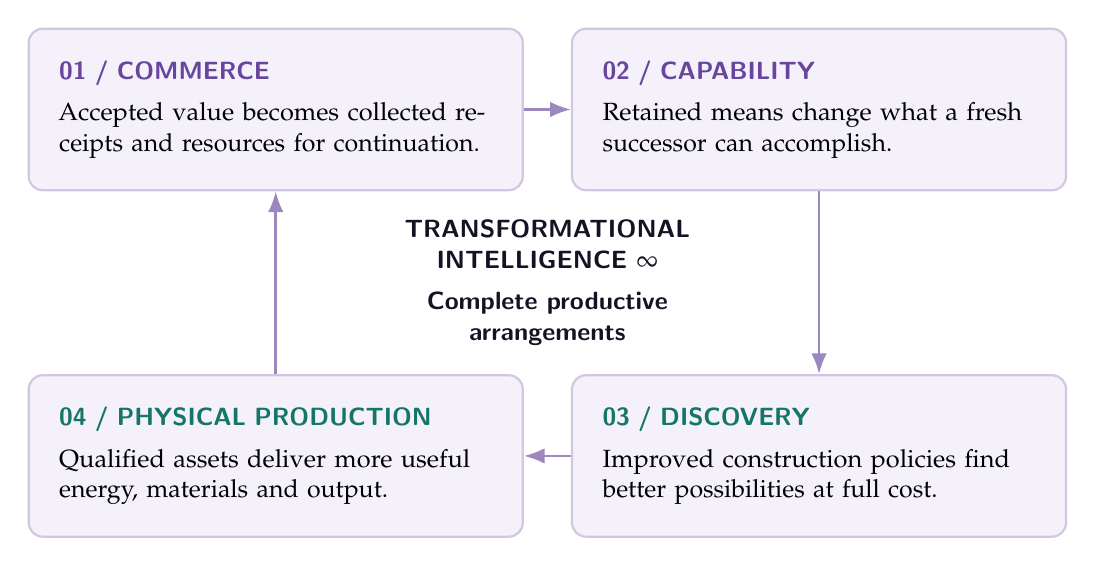
\begin{tikzpicture}[>=Latex,node distance=1.8cm,
box/.style={draw=violet!30,rounded corners=5pt,line width=.8pt,fill=pale,text width=5.5cm,minimum height=2.05cm,align=left,inner sep=11pt,font=\small},
flow/.style={->,line width=1pt,color=violet!65}]
\node[box] (commerce) at (-3.45,2.2) {\textcolor{violet}{\sffamily\bfseries 01 / COMMERCE}\\[4pt]Accepted value becomes collected receipts and resources for continuation.};
\node[box] (capability) at (3.45,2.2) {\textcolor{violet}{\sffamily\bfseries 02 / CAPABILITY}\\[4pt]Retained means change what a fresh successor can accomplish.};
\node[box] (physical) at (-3.45,-2.2) {\textcolor{mint}{\sffamily\bfseries 04 / PHYSICAL PRODUCTION}\\[4pt]Qualified assets deliver more useful energy, materials and output.};
\node[box] (discovery) at (3.45,-2.2) {\textcolor{mint}{\sffamily\bfseries 03 / DISCOVERY}\\[4pt]Improved construction policies find better possibilities at full cost.};
\node[align=center,text width=5.6cm,font=\sffamily\bfseries\small,text=ink] (core) at (0,0) {TRANSFORMATIONAL\\INTELLIGENCE $\infty$\\[4pt]Complete productive\\arrangements};
\draw[flow] (commerce.east)--(capability.west);
\draw[flow] (capability.south)--(discovery.north);
\draw[flow] (discovery.west)--(physical.east);
\draw[flow] (physical.north)--(commerce.south);
\end{tikzpicture}
\end{center}

\vspace{3mm}
{\small\textbf{Figure~\thefigure.} Four processes can reinforce one another. Each has its own measured outcome. The arrows are hypotheses to establish in a particular enterprise; a successful loop does not certify the other three.}

\vfill
\textbf{Research continuity.} This is a distinct manuscript in the AGI ALPHA collection. It follows \emph{Transformational Intelligence: Learning to Change the Game}, the AGI ALPHA foundation, the OUT papers, \emph{Invent the Economy}, \emph{Beyond the Production Frontier} and the November flywheel papers \cite{ti,foundation,economy,frontier,flywheel11,report20261102}. Earlier editions and their experimental outcomes remain unchanged. Public repository evidence is pinned to \nolinkurl{030de783ae67e9a9a2330264a099740c50740f87}; original studies retain their own earlier source identities.

\clearpage
\section{The industry is an invention}
An organization that can cheaply answer existing questions is useful. An organization that can construct a new way to observe, manufacture, coordinate or verify can change which questions and enterprises are worth pursuing. A reusable scientific instrument can turn a bespoke investigation into a repeatable service. A new acceptance method can make an otherwise unfinanceable production commitment credible. A complementary manufacturing process can make an abundant material useful where it was previously unsuitable. In each case, intelligence changes the means of creating value.

SUPER ALPHA names the ambitious economic consequence: a valuable activity becomes attainable, its producer develops a substantial and renewable advantage, and the resulting surplus and capability help create something more powerful. The activity might be a service, a production process, an experimental interface or an industry that does not yet have an established category. Its importance is determined by the outcomes it makes possible, the people who voluntarily benefit, and the resources it consumes.

This viewpoint extends the project from optimizing a supplied business to inventing the conditions under which a better business can exist. Transformational Intelligence treats representations, observations, coordination and intermediate objectives as design variables while preserving the authorized purpose \cite{ti,original}. \emph{Invent the Economy} applies that freedom to viable exchange \cite{economy}. The missing means can therefore be technical, institutional or a combination. A known algorithm inside a new complete arrangement may be decisive. A novel algorithm with no acceptable complete use may have little immediate economic consequence.

\subsection{Three questions that must meet}
The first question is constructive: \emph{what can we make possible?} The second is economic: \emph{why will participants choose it, and what surplus can sustain its producer?} The third is recursive: \emph{what does success enable next?} Their answers have to connect in the same arrangement. A distant market-size estimate cannot supply a missing instrument. A correct instrument cannot supply a missing buyer. A profitable first sale cannot establish an improved invention process.

The relevant historical insight is modest but powerful: the set of useful economic activities changes when technology and organization change. Endogenous-growth theory makes investment in nonrival, partially excludable ideas part of economic growth itself \cite{romer}. Innovation strategy explains why the creator of a technology may capture little of its value when complementary assets and imitation determine who benefits \cite{teece}. SUPER ALPHA brings those questions into an executable invention program: search over the productive means and the arrangements that allow useful invention to continue.

The research aspiration is enormous. Scientific capability could become a reproducible productive asset. Better instruments could make better manufacturing methods attainable; manufacturing could lower the cost of new instruments and energy systems; those assets could support yet more demanding discovery. At sufficiently advanced stages, the relevant frontier includes construction and productive infrastructure beyond Earth. Every transition requires an actual capability, suitable resources and validated performance. A compelling trajectory begins with a discriminating present-day construction.

\subsection{A definition with consequences}
\begin{definition}[SUPER ALPHA research objective]
Construct a consequential expansion of economically attainable outcomes, establish a substantial advantage under a stated complete comparison, and demonstrate a repeatable connection from accepted delivery to retained resources and successor productive capability.
\end{definition}
The term denotes a research and enterprise objective. It is not a measured financial alpha, a guarantee of returns, an attained intelligence classification or a theorem that every invention must be profitable. Commercial success, scientific invention and physical expansion can each be valuable separately. A claim to their complete combination requires evidence for the connections.

\section{Invent the complete productive arrangement}
Let an arrangement be
\begin{equation}
a=(y,m,v,g,f,\pi),
\end{equation}
where $y$ is the valuable outcome, $m$ the production means, $v$ the acceptance and evidence method, $g$ the agreements and allocation of risk, $f$ the financing terms, and $\pi$ the operating policy. During opportunity discovery, the enterprise may propose a new outcome and a different arrangement. Once an outcome enters a comparison, its required beneficiary purpose and legitimate constraints remain fixed while the means are transformed.

For example, a buyer may need a reliable decision about a manufactured part. The inherited method might require reconstructing every hidden physical variable. A new measurement could supply the missing information. Alternatively, a different decision procedure could identify exactly the sufficient observable, making full reconstruction unnecessary. Both are legitimate constructions if the original decision, reliability and service obligations are preserved. Relabeling an easier output as the requested result is not such a construction \cite{original,world,outlearn}.

\subsection{Find the freedom inside the obstacle}
Useful intervention begins by classifying a restriction. Some restrictions are physical facts or commitments. Others are uncertain assumptions. Still others are consequences of the current method. This distinction changes the design space. An inaccessible sensor may motivate a new sensor, a substitute observable, a process that makes the nuisance constant, or a production method that avoids the nuisance entirely.

The same reasoning applies to economics. A customer may be unable to justify building a specialized instrument alone while a group of customers can share its fixed construction burden. A producer may be able to deliver only after a staged contract resolves working-capital timing. A product may become viable through a different acceptance boundary that avoids repeated whole-system inspection. The construction must include the new coordination, enforcement and maintenance costs. These changes follow the earlier papers' central discipline: an inherited prerequisite of one method need not be a prerequisite of the desired outcome \cite{economy,outdesign,outexecute,outaccelerate}.

\subsection{Transfer structure and construct its missing connector}
Analogy becomes useful when it preserves the causal structure needed for an outcome. Map entities, relations, invariants, disturbances and acceptance conditions. At a mismatch, construct an adapter, obtain the missing observation, change the formulation or reject the transfer. Vocabulary similarity is weak evidence. Structure-mapping theory supplies a basis for the comparison; an actual executable adaptation supplies the engineering test \cite{gentner}.

A successful adaptation should leave more than a story. Retain the instrument, its input contract, its limits and the procedure that constructs or adapts it. A reusable artifact performs a task. A constructor produces a family of artifacts. A better discovery policy finds useful constructors or arrangements more effectively. These are different objects, with different comparisons \cite{outevolve,flywheel11}.

\subsection{Design an environment in which less reasoning is necessary}
An enterprise can improve by making relevant facts observable and valid work easier to check. Versioned interfaces, calibrated fixtures, typed transformations and complete dependency records can reduce the need to reconstruct the same reasoning repeatedly. This is a concrete source of acceleration: production carries the evidence that future decisions need. Its value is measured after the cost of constructing, using and maintaining that environment \cite{world,outthink,outreflect,outaccelerate}.

This perspective matters for scale. Repeating a costly reasoning process millions of times can be inferior to constructing a process that removes its recurring cause. Whether that construction pays depends on the actual reuse horizon, changing requirements and the cost of invalidation. A specialized environment can also create a new blind spot; fresh acceptance must remain sensitive to conditions outside its contract.

\section{Economic possibility is a scoped, testable claim}
\subsection{Separate physics from the operational frontier}
An invention does not alter the laws of physics. If a theoretical feasible set already includes every physically possible future construction, the invention was already inside that set. Calling it an expansion of that omniscient set would be a category error.

The operational frontier is conditioned on information, available means and the resources required to discover, construct and deploy a complete route. Let $d$ declare the purpose, workload, quality, deadline, rights, information, financing opportunities, risk obligations and resource envelope. Let $\mathcal B_d$ contain the strongest feasible comparison routes, including competent adaptive construction and permitted coordination. A routine fixed baseline is insufficient when a conventional constructor could build the same solution.

For a tested route $b$ and outcome $y$, write $E_d(b,y)=1$ only when the complete route meets the declared technical, participation, funding and service conditions. Record a failed condition as $0$ and an untested material condition as unknown. An unknown comparator does not count as a defeated comparator.

\begin{definition}[Tested economic enablement]
Choose a named, nonempty tested subset $\mathcal B_d^{\rm test}\subseteq\mathcal B_d$. A construction exhibits economic enablement relative to $(d,\mathcal B_d^{\rm test})$ when $E_d(a,y)=1$ and $E_d(b,y)=0$ for every $b\in\mathcal B_d^{\rm test}$. Each failure must identify a required condition under the matched envelope. Material untested alternatives leave the claim over the broader $\mathcal B_d$ unresolved.
\end{definition}
This is a claim about the examined information and complete alternatives. It does not prove that no person, firm or future algorithm could have produced the outcome. A broader claim of unprecedented economic feasibility needs correspondingly broader historical and market evidence. Conversely, failure to establish uniqueness does not erase a useful construction or ordinary commercial profit.

\subsection{Five conditions define an economically usable route}
\textbf{Acceptance.} The complete beneficiary outcome meets its independently defined purpose, quality, deadline and future service obligations. Changing the instrument requires checking that its acceptance semantics remain appropriate.

\textbf{Voluntary participation.} Every necessary participant receives at least its outside-option utility under the modeled information and risk allocation. Buyers may decline, self-produce, choose a rival or defer. Suppliers and capital providers also have alternatives. A positive aggregate surplus does not prove that a feasible transfer and commitment scheme exists; classical bilateral-trade impossibility results illustrate the constraints introduced by private information and incentive compatibility \cite{myerson}.

\textbf{Complete resources.} Search, construction, unsuccessful attempts, acquisition, production, verification, support, financing, maintenance and residual obligations are included. The reference and candidate receive equivalent permissions to invent, reuse and coordinate. An economic resource cost can exist even when its execution uses an included subscription capability.

\textbf{Timed funding.} Each commitment is feasible with actual available funds at that time, after protecting obligations and declared reserves. A future invoice, valuation or possible investment is not money available for an earlier purchase. A separately modeled financing arrangement must state who supplies funds, when, and on what voluntary terms.

\textbf{Continuity.} The operating policy can maintain the relevant service and resources across the declared horizon. A short profitable cohort with an unfunded warranty tail does not establish a sustainable delivery arrangement. Durability is tested under its stated changes in demand, rivals, suppliers and operating conditions.

\subsection{A useful scalar witness}
Fix one coalition boundary and workload. Let $W$ be aggregate beneficiary value relative to outside options, and let $C$ be the complete real resource and supplier opportunity burden, counted once within that boundary. Internal transfers are excluded from both quantities. The scalar $W-C$ is an initial surplus screen; the enterprise's cash expenses and profit are a separate accounting view. When $W<C$, no rearrangement of payments among those participants can cover the deficit without an additional benefit, subsidy, cost reduction or changed scope. When $W>C$, technical acceptance, incentives, allocation of surplus and funding timing still require construction.

\begin{proposition}[The surplus screen]
Under quasilinear utility, the stated benefits and complete resource costs, voluntary transfers that cover costs require nonnegative total surplus. Positive total surplus alone does not establish implementation with private information, restricted transfers or liquidity constraints.
\end{proposition}
\begin{proof}
Sum each participant's utility relative to its outside option. Transfers within the arrangement cancel, leaving benefits minus resource costs. If that total is negative, at least one necessary participant must receive negative incremental utility. Restrictions on feasible transfers, information and time can prevent implementation even when the summed inequality is positive.
\end{proof}
The proposition is a basic accounting and participation condition. The contribution of this paper is to connect it to invention, rival response and successor construction, rather than to claim a new general welfare theorem.

\section{Create value and construct the means to retain it}
\subsection{The advantage must survive the market it helps create}
A technical breakthrough can make buyers substantially better off while leaving its inventor unable to recover construction costs. Others may copy the method, control distribution, own a scarce complementary asset or offer a sufficient substitute. Teece's account of appropriability and complementary assets makes this separation explicit \cite{teece}. SUPER ALPHA therefore treats value capture as part of the productive arrangement.

Sources of an earned advantage include a lower complete delivery cost, better calibrated evidence, shorter qualification time, reliable access to scarce inputs, cumulative operational knowledge, a difficult-to-reproduce constructor, and superior service across changing requirements. Each can erode. Record what is scarce, how a rival could obtain it, what it costs to maintain, and which buyer outcome the advantage improves. Ownership of an intellectual artifact alone is an incomplete answer.

The healthiest recurring advantage can be the ability to renew the productive frontier: while competitors reproduce one outcome, the enterprise constructs another that is useful and harder to deliver with the previous means. This is a hypothesis about the relative pace and cost of construction, qualification and adoption. It requires fresh measurements. It cannot be inferred from agent count, a long library or a claim of unlimited intelligence.

\subsection{Keep the commercial window open}
For a homogeneous, accepted cohort of $n>0$ buyers, let $w$ be each buyer's value net of its best outside option, $F$ the complete fixed burden, $c$ the variable cost and $r$ a stated ceiling imposed by competitive response. To earn at least $m>0$ while giving buyers strictly positive surplus, an implementable price must satisfy
\begin{equation}
\frac{F+m}{n}+c\ \le p\ \le r,\qquad p<w.
\end{equation}
The elementary price window is nonempty exactly when its lower endpoint is no greater than $r$ and strictly below $w$. A production invention can lower the endpoint; shared construction can spread $F$; better evidence can change a justified buyer value or risk burden; competition can lower the ceiling. The outcome and its commercial arrangement therefore determine viability together.

This screen assumes the declared costs, values, quantity and price-response rule. It supplies neither an incentive-compatible multi-party contract nor a solution to entry, financing or market discovery. In a real enterprise, each parameter has to be observed, contracted or represented as an explicit uncertain hypothesis. The window can close after a successful first sale.

\subsection{Turn the shortfall into a specification for invention}
The commercial window also identifies a concrete construction target. For a prospective route with $w>r$, define the shortfall against desired profit $m$ as
\begin{equation}
\Delta=F+nc+m-nr.
\label{eq:construction-gap}
\end{equation}
If $\Delta>0$, the current complete arrangement cannot earn $m$ at a permitted price. Holding the outcome, cohort and ceiling fixed, an accepted construction must remove at least $\Delta$ of complete cost. Alternatively, it must establish a different viable arrangement or enough additional voluntary demand with qualified capacity. The burden of discovering and building the change belongs in the revised costs.

For example, take $F=30$, $c=7$, $n=10$, $r=10$, $w=13$ and $m=20$. Current cost is 100, allowable cost is 80, and the gap is 20. Three conditional design targets follow:
\begin{center}\small
\begin{tabularx}{\linewidth}{@{}P{3.2cm}P{2.1cm}Y@{}}\toprule
Construction direction & Target & What must be established\\\midrule
Reduce the fixed burden & $F\le10$ & A complete construction and qualification route at that burden.\\
Reduce marginal burden & $c\le5$ & Accepted delivery, including checking and corrections, at that cost.\\
Expand the cohort & $n\ge17$ & Additional willing demand, capacity and timed funds; a newly scoped workload.\\\bottomrule
\end{tabularx}\end{center}
Each row varies one term while holding the other stated terms fixed. These targets are deductions from the authored model, not achieved cost reductions or market demand. Previously incurred costs remain in the enterprise history.

\textbf{Economics specifies the change; invention constructs the means.} Search backward from the threshold to a missing observation, process, interface or agreement. Search forward from a newly constructed means to further valuable uses. A target becomes an opportunity only when an executable route can meet it. This converts a failed business inequality into a disciplined question about what to invent.

\subsection{Renew the advantage before its resources run out}
A durable enterprise must recover its construction burden and retain enough available resources to qualify its next useful means as its current advantage erodes. Measure the time to accepted construction, the time and cost for a competent rival to reproduce it, the customer's adoption and renewal cycle, and the cash available after service obligations. Compare a policy that renews the means with a strong policy that exploits current capabilities, licenses a substitute or retains cash.

Faster invention helps only when the resulting successor has a valuable accepted use. A slower construction can remain worthwhile if existing earnings bridge its cost and delay. The decisive object is a feasible sequence of accepted, funded commitments under evolving alternatives, not a fixed ratio between two uncertain clocks. This succession test gives renewable advantage a causal meaning without assuming permanent monopoly or automatic exponential growth.

Growth theory already connects anticipated future innovation to the erosion of present innovation rents and research incentives \cite{aghionhowitt}. For a particular enterprise, the connection becomes a question about the dates of collections, construction and qualification.

\begin{proposition}[A funded renewal window]
\label{prop:renewal}
In a declared deterministic scenario, let an already qualified route generate nondecreasing cumulative unrestricted settled surplus $M(t)$, with $M(0)=0$. Initial available cash is $U_0\ge0$. A successor requires an upfront amount $K\ge0$, takes qualification time $\tau\ge0$, and must qualify by a latest useful date $T\ge0$. Assume its complete qualification path is feasible, its upfront amount covers that path, and construction does not interrupt the predecessor's stated surplus. With no additional financing, a funded timely start exists exactly when
\begin{equation}
\tau\le T\quad\text{and}\quad K\le U_0+M(T-\tau).
\label{eq:renewal-window}
\end{equation}
\end{proposition}
\begin{proof}
A timely start has $s\le T-\tau$. Monotonicity gives $M(s)\le M(T-\tau)$, so funding requires the stated inequality. Conversely, when it holds, starting at $T-\tau$ is funded and qualifies at $T$.
\end{proof}
For constant settled surplus rate $\mu>0$, the earliest qualification date is
\begin{equation}
t_{\rm qualify}=\frac{(K-U_0)_+}{\mu}+\tau,\qquad (x)_+=\max(x,0).
\label{eq:qualification-time}
\end{equation}
It must be no later than $T$. At zero surplus rate, upfront funding must already be available and $\tau\le T$. The date $T$ must come from a declared opportunity and response scenario; it is not inferred from a general promise of imitation. This result tests the funding and calendar of a proposed renewal. Its value and advantage still require the commercial comparison. Lumpy payments, changing reserves or interrupted production use the ordered cash condition below. An operating commitment uses funds that have actually settled at its start.

\subsection{Specify the game before claiming an optimum}
Let $r$ denote a rival, supplier and buyer response, and let $\Pi_H(a,r)$ denote complete-cost profit over a declared horizon $H$. A robustness screen can ask whether
\begin{equation}
\underline\Pi_H(a)=\inf_{r\in\mathcal R_d}\Pi_H(a,r)>0,
\end{equation}
for a disclosed set $\mathcal R_d$ of supported responses, subject to participation, quality and cash constraints. This is conditional robustness over the declared set. It is not robustness to every possible response or an equilibrium proof.

If the question is game-theoretic optimality, specify the players, information, timing, feasible actions, transfers, response rule and objective. Then solve that game or report an approximation gap. An assumed fixed rival price cannot establish a monopoly rent that would survive entry. A best response inside a finite menu cannot establish the best enterprise among all possible industries.

The design choices themselves may change the game. A shared instrument, interoperable interface, outcome-based contract, license or staged commitment can alter cost and participation. Compare the new game with the best permitted alternative arrangement, including its own financing and coordination. Changed rules should create useful cooperation and accepted output; coercive dependence and unpriced external costs are not evidence of productive advantage.

\subsection{Capture enough to renew; preserve the customer's reason to choose}
The objective is sustained, growing value creation with viable producer returns. A high nominal price is valuable only if it remains voluntarily acceptable and collectable. A low price can accelerate adoption but destroy the resources needed to maintain quality or invent successors. The correct choice depends on the measured demand, cost, risk and competitive environment.

Useful arrangements can divide value among the inventor, operators, complementary suppliers and beneficiaries. Broad adoption can increase total value even when the inventor retains only a fraction. That fraction must be earned through a service, right or contribution others choose to pay for. Customer savings, ecosystem value, asset valuation and enterprise profit are distinct quantities; adding them together exaggerates success.

\section{Four processes must earn their own compounding claims}
\subsection{Commerce creates resources for continuation}
The commercial loop converts accepted delivery into collected receipts, covers complete costs and protected obligations, and makes a subsequent commitment affordable. The relevant state includes unrestricted cash, receivables, liabilities, productive assets and remaining service duties. Profit is a period result; cash is a dated stock. A sound report reconciles them without treating a reserve as an additional expense or counting both full capital expenditure and its depreciation as the same period's cost.

Define the available amount at time $t$ as $U_t=C_t-R_t$, where $C_t$ is cash and $R_t$ denotes nonoverlapping amounts reserved for existing obligations. A new commitment $I_t$ requires $U_t\ge I_t$ under the declared policy. Financing can increase available resources while adding repayment, dilution or other obligations. It does not become revenue or earned profit.

\begin{proposition}[The capital required by a complete sequence]
\label{prop:capital}
Fix a technically and contractually feasible plan with ordered events $j=0,\ldots,J$. Let $P_j$ be cumulative cash payments, $S_j$ cumulative settled nonfinancing receipts, $L_j$ cumulative financing actually received, and $R_j$ required protected cash immediately after event $j$. Event zero includes any opening reserve. The least opening cash satisfying every cash-protection constraint is
\begin{equation}
C^\star=\max\!\left(0,\max_{0\le j\le J}\{R_j+P_j-S_j-L_j\}\right).
\label{eq:capital}
\end{equation}
\end{proposition}
\begin{proof}
At each event, the requirement is $C_0+S_j+L_j-P_j\ge R_j$. Rearranging all these inequalities and imposing $C_0\ge0$ gives exactly $C_0\ge C^\star$.
\end{proof}
Receipts, payments and reserve changes have explicit event order; a later receipt cannot fund an earlier payment merely because both share a calendar date. The plan includes financing terms, repayments and remaining service duties over its stated horizon. Its fixed funding path cannot depend on spending money before it is received. Comparing prospective plans by complete profit, $C^\star$ and qualification time makes capital and the choice of productive means part of the same design decision. The identity is a cash-feasibility deduction for the declared plan, not a claim that its demand, qualification or funding has been secured.

\subsection{Capability inheritance changes what a successor can do}
The capability loop retains a useful instrument, representation, constructor or production process and applies it to fresh work. Its result may be a new accepted output, lower complete cost, greater reliability or a shorter route to acceptance. A causal comparison removes or substitutes that inherited means while preserving the relevant starting resources.

Distinguish \emph{financed by}, \emph{enabled by} and \emph{used by}. An earlier profit may pay for an ordinary successor that anyone with the same money could buy. An earlier instrument may enable a successor that available money alone cannot construct within the declared deadline. A successor may use an inherited asset without improving its result. All three relations are informative; they support different claims \cite{outevolve,flywheel11}.

\subsection{Discovery improvement makes better construction more likely}
The discovery loop changes the procedure that selects, constructs and tests possibilities. Its natural precedent includes program-library learning and archive-based agent improvement, each within its own evaluated domains \cite{dreamcoder,dgm}. A new library can improve task performance while leaving the discovery procedure unchanged.

To separate these effects, cross old and new discovery policies with old and new starting capabilities. Let $Y_{ij}$ be an accepted outcome measure, after the declared cost treatment, for policy $i$ and asset condition $j$. One concrete choice is the fraction of a fixed, preregistered request population independently accepted by a common endpoint within the same complete campaign budget. Failed, declined and unfinished requests remain in its denominator; report complete costs and outcome value alongside that fraction. Estimate the policy effect within each fixed asset condition and the asset effect within each fixed policy. The interaction
\begin{equation}
\Delta_{\mathrm{int}}=Y_{11}-Y_{10}-Y_{01}+Y_{00}
\end{equation}
describes complementarity in this design. It does not alone identify why improvement occurs. Include equal-content ordinary reuse, strong adaptive conventional search, failed attempts and acquisition costs. Fresh tasks should test changed demands, not only familiar templates.

\subsection{Physical production expands qualified productive capacity}
The physical loop converts resources and designs into commissioned assets that deliver useful output. Relevant outcomes include net useful energy, conforming throughput, yield, reliability, measurement capability, lifecycle material consumption and maintenance burden. Qualification and replication lead times matter. A larger bank balance, a digital twin or a simulated factory does not measure these outcomes \cite{frontier}.

The processes can complement one another. Better instruments may reduce qualification cost. Better qualification may improve financeability. Reliable production may generate surplus and new observations. Those observations may improve constructors. The evidence must follow the actual arrows. A successful commercial loop is useful even if the discovery loop does not improve; a scientifically valuable instrument remains useful before it generates a sale.

\Needspace{8\baselineskip}
\section{A practical architecture for transformational invention}
\subsection{Search from consequences, then construct backward}
Begin with a valuable activity that current complete methods struggle to deliver. Compare materially different possibilities before committing to a construction. Ask which limitation matters most: unavailable information, incompatible components, a costly acceptance method, an unworkable division of risk, scarce capacity or a prerequisite that the beneficiary never needed.

Construct the smallest executable intervention that could change the decision. Its description includes allowed inputs, prerequisites, operations, outputs, effects, verification, costs and conditions for stopping or revision. A broad ambition is compatible with a small decisive test. A narrow test is valuable when its success would unlock a consequential class of work.

Search forward as well as backward. A newly calibrated instrument, cheaper material process or reusable constructor may enable a valuable activity nobody specified before that capability existed. Ask what outcomes are now attainable, which beneficiaries would value them, and what additional connector would make them economical. Then test that newly proposed purpose and its voluntary demand. This forward step prevents a fixed list of services, benchmarks or imagined industries from becoming the permanent boundary of the search.

\subsection{Use criticism to produce a better observation or design}
A critic should identify an exact contradiction, omission, counterexample or discriminating test. Adjudicate the objection against the source and the unchanged purpose before repairing the proposal. When several explanations fit, consider that all may be incomplete. The next action may acquire information, construct a new instrument, take a robust acceptable action, eliminate the uncertain dependency or stop the attempt.

The verification method is also a construction with failure boundaries. Carry provenance and dependence information into the output, then challenge whether those records omit a relevant condition. Agreement among agents is not an independent observation. Source consistency is not external truth. Separate proposer, checker and authority at the level required by the consequence \cite{outreflect,enterprises,foundation}.

\subsection{Retain the next starting point}
Keep the useful artifact, its constructor when available, its applicability conditions and the concise lesson from failure. Retention should reduce future construction or verification burden. A collection of transcripts does not automatically do so. Invalidation conditions are part of the asset: changed sensors, objectives, material regimes, rights or service obligations can require new qualification.

Knowledge should be retained separately from execution permission. A successor can inherit a method without inheriting authority to spend, contact a customer, control equipment or change its own acceptance standard. This separation permits ambitious reuse while keeping each new commitment accountable \cite{enterprises,foundation}.

\subsection{Choose continuation jointly with capital and opportunity}
The next action may repeat a profitable delivery, acquire a customer, improve a constructor, build a complementary instrument, expand capacity or retain cash. There is no universally optimal fixed research percentage. Compare relevant consequences, timing, uncertainty and outside options. When probabilities lack a basis, expose the scenarios and the decision boundary rather than manufacture a precise expected value.

The AGI ALPHA implementation already provides canonical enterprise accounts and operating boundaries; this paper adds no parallel ledger or autonomous deployment authority. Its analytical companion is an inspectable calculation. Any operational adoption must use the existing account, acceptance and authorization paths with a fresh source-bound qualification.

\section{An exact illustrative economy}
\label{sec:example}
The following construction is deliberately authored to expose logical distinctions. Its values are abstract units, its buyers are stipulated and its acceptance cases are supplied. It is not an estimate of a market, a new autonomous invention or a native enterprise simulation. The supplied program uses exact arithmetic and emits the complete scenario table.

\subsection{Production and coordination are complementary}
Ten buyers each value one accepted output at 13 units. A selected price of 12 leaves each buyer one unit of incremental benefit. The old production method has fixed construction cost 20 and variable cost 12 per output. The new method has fixed cost 30 and variable cost 7. Independent construction repeats the fixed cost for every buyer; pooled construction pays it once. The aggregate fixed and variable costs include all burdens \emph{inside this authored model}. No inference about real acquisition, legal, compute or support costs follows.

\begin{table}[htbp]\centering\small
\begin{tabularx}{\linewidth}{@{}Yrrrr@{}}\toprule
Complete arrangement & Cost & Receipts & Profit & Max. surplus\\\midrule
Old method, individual construction & 320 & 120 & $-200$ & $-190$\\
New method, individual construction & 370 & 120 & $-250$ & $-240$\\
Old method, pooled construction & 140 & 120 & $-20$ & $-10$\\
New method, pooled construction & 100 & 120 & $+20$ & $+30$\\\bottomrule
\end{tabularx}
\caption{Conditional delivery economics at the selected price. ``Max. surplus'' is total stipulated value 130 minus complete model cost. Negative rows are forced-delivery diagnostics; a rational optional-entry policy may decline them and earn zero. No sale is inferred when a required condition fails.}\label{tab:arrangements}
\end{table}

The production improvement alone raises total cost because its larger fixed burden is repeated. Pooling alone cannot cover the old method's cost even at total willingness to pay. Joint construction costs 100, generates 120 in collected receipts under the accepted scenario, and leaves 20 profit plus 10 buyer benefit. The 30 units of total surplus match the participation identity.

A strong conventional constructor allowed to use the same production and pooling choices selects exactly this joint route. It ties cost, acceptance and profit. The example establishes complementarity within the declared choices, while providing no unique advantage for the SUPER ALPHA label or discovery procedure. Relative to that complete comparator, the tested economic-enablement residual is zero.

\begin{figure}[htbp]\centering
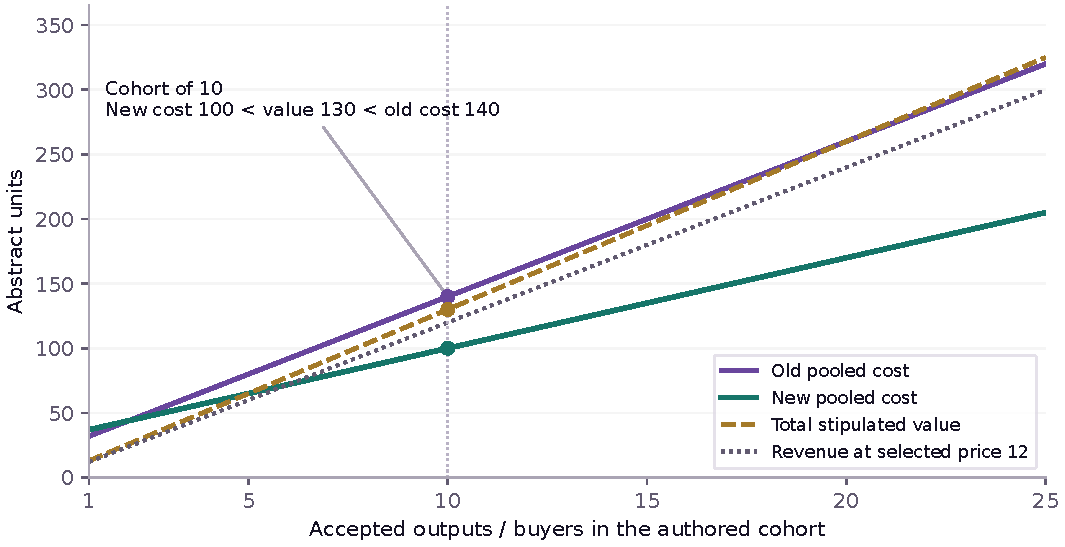
\includegraphics[width=.91\linewidth]{figures/thresholds.pdf}
\caption{Exact cost boundaries for the authored pooled methods. Workload changes the conclusion: old pooled delivery becomes affordable at a larger cohort if its price can rise above 12 while remaining below 13. At ten buyers, new pooled cost is 100, old pooled cost is 140, and total willingness to pay is 130. The selected-price revenue line is separate from willingness. This is a conditional model boundary, not market demand evidence.}\label{fig:thresholds}
\end{figure}

\FloatBarrier
\subsection{Change one condition and the apparent flywheel can break}
At five buyers, the new pooled method costs 65 and the selected-price receipts are 60, producing a loss of five. At value nine per buyer, even total willingness of 90 cannot cover the ten-buyer cost of 100; the original price is rejected. A predeclared acceptance failure can consume the 100 cost while producing no accepted revenue. These outcomes remain in the supplied result set.

For a collection-delay example, begin with 100 units of actual equity, spend the 100 operating cost, accept delivery and recognize an invoice of 120 that is not yet collected. Accounting profit is 20, receivables are 120 and cash is zero. A successor requiring cash must wait or obtain a separately accepted financing arrangement. The positive profit result remains intact.

After collection, cash is 120. If 15 is protected for a contingent service obligation under the model policy, only 105 is unrestricted. A successor requiring 110 remains unaffordable. Reserving 15 changes availability; the model does not charge the reserve again as an expense. If an obligation becomes an incurred cost, recognition and cash treatment must follow its actual terms.

\subsection{The same profit can require different capital and miss renewal}
Extend the existing example with the stipulated successor payment of 110 and accepted, collected successor receipt of 145. Total receipts are 265, total expensed and paid costs are 210, and complete-history profit is 55 in each completed scenario. Apply Proposition~\ref{prop:capital} to the full ordered sequence:
\begin{center}\small
\begin{tabularx}{\linewidth}{@{}YP{2.25cm}P{2.15cm}@{}}\toprule
Collection and protection schedule & Required opening cash $C^\star$ & Complete-history profit\\\midrule
Collect 120 before paying 110; no reserve & 100 & 55\\
Accept and collect 120, then protect 15 and pay 110 & 105 & 55\\
Accept the first invoice and protect 15; pay 110 before collecting 120 & 225 & 55\\\bottomrule
\end{tabularx}\end{center}
Every case first pays the predecessor's 100. In the second case, first acceptance and collection occur together before the reserve is required; in the third, acceptance creates a protected obligation before collection. The protected amount remains held through the illustrated successor; any later realized service cost would be a further expense and payment. The second sequence reaches its largest protected deficit after the successor payment: $15+210-120=105$. The third reaches $15+210=225$ before either collection. If protection begins before the first collection but successor payment follows it, the requirement is instead 115. At the original opening cash of 100, only the unreserved schedule can complete as specified. The other profit totals describe feasible completion at their required capital, not earnings obtained by spending unavailable cash.

The calendar supplies a second boundary. In the separate renewal illustration, take initial unrestricted cash $U_0=20$, net settled surplus rate $\mu=10$ per time unit, successor qualification cost $K=60$, qualification delay $\tau=3$ and latest useful date $T=6$. Although 80 is available by date six if no investment is made, a funded construction starts no earlier than date four and qualifies at date seven. The renewal misses its opportunity.

Two conditional changes meet the date-six boundary exactly: starting with 30 available units, or qualifying the same 60-unit construction in two time units. These are different prospective capital or engineering designs. A shorter qualification path must actually preserve acceptance and include its own complete cost. The analytical companion checks these boundaries, zero-surplus cases and event ordering. Retaining cash, exploiting the existing means or licensing a qualified alternative remains eligible; timely renewal alone does not establish which choice produces the best complete outcome.

\subsection{Imitation can transfer value away from the inventor}
Suppose that, after the inventor has spent 30 on the common construction, an equivalent rival can serve this cohort at a price cap of seven. The inventor's maximum contribution from ten sales is then $10(7-7)=0$ before its sunk fixed construction cost, leaving a complete project loss of 30. If that condition is known before entry, non-entry yields zero and dominates the project. If it arrives afterward, the construction loss remains incurred.

This is a declared post-entry competitive scenario, not a derivation of a full entry equilibrium: the rival's source of fixed capability is stipulated and could be inherited from previous work. Its lesson is precise. A large buyer benefit can coexist with no new resources for the original inventor's renewal. A sustainable capture claim needs an explicit source and duration of advantage, or a different voluntarily accepted arrangement.

\subsection{Finance, capability and discovery require different controls}
With 120 in available cash, a successor costing 110 with an inherited means can proceed, while a route costing 130 without it cannot. This is a cost-and-resource enabling witness under the stipulated successor contract. A second successor costing 115 in either condition is merely affordable: the inherited means has no causal cost benefit in that comparison. These commitment comparisons establish affordability under the stated alternatives. For optional reconciliation cases, the companion stipulates accepted and collected successor receipts of 145 and 130, producing complete-history profits of 55 and 35, respectively. These authored receipts provide no evidence of real successor demand or profitable operation.

The discovery negative control crosses old and new policies with old and new assets. Both policies cost 40 without the new asset and 24 with it, for the same accepted result. Acquisition costs 16. One use therefore breaks even on total resource cost; repeated compatible uses may amortize acquisition. The policy effect is zero in both asset conditions. The example demonstrates how saved work can be real while a claim of improved invention remains unsupported.

\FloatBarrier
\section{What the public experiments establish}
The public corpus supplies important constraints on the research program. This section reviews its pinned evidence; it does not claim a fresh replay of every experiment or pool distinct enterprises into one result. The November report preserves complete denominators, source identities and the scope of its own reproductions \cite{report20261102}.

\begin{table}[htbp]\centering\small
\begin{tabularx}{\linewidth}{@{}P{3.0cm}YY@{}}\toprule
Construction & Source-bound result & Consequence for SUPER ALPHA\\\midrule
Instrument foundry & Each arm: 30 accepted programs and 6 nonidentifiability certificates in 36 requests. Conventional compilation uses 13,566 arithmetic operations; accumulating construction uses 48,141. & Retained construction can work while a complete conventional route wins. Tool inheritance and superior discovery need separate evidence.\\
Paired acquisition & 80 material cases and 12 spatial model fields pass; same-information conventional methods tie. Four undetected-error witnesses remain. & A numerical instrument needs calibrated physical qualification and a distinct commercial comparison.\\
Discovery allocation & NEXT072 finds 14 of 24 targets in 23 additional selection queries; strong conventional controls find 15. The complete acquisition accounting is 123 profiles per policy. & Familiar data replay and named mechanisms do not establish a new discovery advantage.\\
Financial portfolio & 110 authored native scenarios complete. Best final trailing-year profit is zero; 23 retain uncovered obligations. & This supplied market does not establish profitable scaling; a different complete arrangement requires new evidence.\\\bottomrule
\end{tabularx}
\caption{Selected public evidence at its original scope. Sources: the foundry edition, paired acquisition record and report \cite{flywheel11,paired,report20261102,r2}. Operation counts, model acceptance and simulated money measure different things.}\label{tab:public}
\end{table}

The financial portfolio also exposes a limit of its supplied opportunity set. Each account has eight authored buyers, at most three purchase opportunities per buyer and a maximum posted price of US\$40,000. Its loose three-year gross-contract ceiling is therefore US\$960,000. No optimizer inside that fixed market can express a US\$3 billion annual-profit route. This is a limit of that experiment, and a reason to construct and test new opportunities rather than assume the original market catalogue defines the economy \cite{r2}.

These findings are useful because they change a decision. Adopt the cheaper conventional compiler when it is appropriate. Repair or avoid an unresolved measurement ambiguity. Search for a different market or production arrangement when the current one cannot support voluntary profitable delivery. Preserve a construction that remains useful even when its motivating advantage claim fails.

Other source-reviewed scenarios in the report include conditional positive modeled profit and earned-funded incremental resources. They have separate accounts, cost assumptions and collateral conditions. Their existence does not contradict the zero best outcome in the distinct 110-account portfolio, nor does it combine into a scalable enterprise. The exact source and account matter more than the largest number in a collection \cite{report20261102}.

No result in this paper establishes observed customer revenue, an improved general discovery procedure, physical industrial expansion or the US\$3 billion milestone. The evidence supports a more targeted next question: which important outcome can a new complete arrangement deliver, and which decisive observation would distinguish it from the strongest existing route?

\section{Three industries worth trying to make possible}
The following are proposed opportunity families. Their commercial novelty, available supply and demand require current research in the specific application. They illustrate the kind of consequence worth pursuing, rather than a claim that these industries have been invented here. Each begins with a missing means and a test whose outcome would change a decision.

\subsection{Scientific capability foundries}
\textbf{The valuable activity.} A customer requests a new, reusable experimental capability: an instrument or interface that can answer a family of consequential questions to an agreed standard. The deliverable includes the working construction, calibration, limits and a demonstrated second use. This can make specialized scientific work economical at a smaller volume or shorter qualification horizon.

\textbf{The missing means.} Turning an open question into a reliable observation often requires coordinated design of fixtures, measurement, models, controls and acceptance. A general-purpose agent that produces a plausible design does not supply the complete capability. A foundry would construct the connector between a scientific purpose and an economical, independently checkable experimental interface \cite{world,outlearn,flywheel11}.

\textbf{The commercial construction.} Candidate arrangements include paid capability development, shared qualification across consenting users, instrument access, validated adaptation and maintenance. The customer buys an accepted capability or service. Pricing and responsibility must reflect failed qualification, calibration drift, rights, support and task-specific revalidation. Capture might come from constructors and operational reliability; its durability must survive competent laboratories, contract research services and other AI-enabled providers.

\textbf{The decisive experiment.} Choose one consequential measurement that a strong complete route cannot presently deliver within a declared budget and acceptance contract. Construct the proposed means. Test it on reference truth hidden from the builder where feasible, include adversarial nuisance cases, and ask an independent user to use it for a changed second question. Compare ordinary shared engineering and the same retained artifacts. Cost both uses, including failures and all human intervention.

\textbf{What success could enable.} A validated instrument can become a component in a more demanding instrument or manufacturing process. The next study must identify that dependence and test the complete successor. A succession of such constructions could turn research capability itself into a repeatable productive asset. Demonstrating that the foundry becomes a better inventor requires the additional discovery-policy comparison.

A concrete proposed lineage begins with an instrument that distinguishes a local material condition the current observation cannot identify. If qualified, it supports an accepted manufacturing decision; that decision can justify a production service whose receipts sustain instrument maintenance and adaptation. The retained observation constructor may then qualify a different process or help build a more capable instrument. The lineage becomes a flywheel only when those successor effects, payments and full costs are independently established. Its first decisive test is the unresolved observation, not a forecast of the later factory.

\subsection{On-demand historical observation}
\textbf{The valuable activity.} A user asks about a past condition that nobody explicitly measured at the required time or resolution. A system constructs a defensible observation series from available traces, with resolution limits, uncertainty and provenance. Potential applications include industrial histories, environmental exposure and the consequences of changes in a production process. A reconstructed series is useful only if it resolves the user's actual decision.

\textbf{The missing means.} Diverse records may constrain a latent historical variable without uniquely identifying it. The system must discover a valid observation operator, establish calibration where possible, and distinguish identification from attractive fit. Additional records can fail to resolve an ambiguity if they observe the same uninformative direction. The earlier optical and manufacturing work makes that failure mode concrete \cite{paired,report20261102}.

\textbf{The commercial construction.} A service could sell a validated retrospective measurement and its defensible uses. Rights to source material, reproducible extraction, updates, liability and an explicit unavailable-result outcome belong in the contract. Buyer value depends on an improved decision, not the length of a reconstructed dataset. Rival alternatives include existing remote sensing, conventional statistical reconstruction, expert analysis and choosing an action robust to uncertainty.

\textbf{The decisive experiment.} Hide independently measured historical truth, freeze the available record sources and extraction cutoff, then reconstruct a preregistered series. Test out-of-distribution events and alternative latent histories that fit the same records. Evaluate a consequential decision with and without the result. If the necessary variable is not identifiable, return the ambiguity or construct the smallest additional measurement that would distinguish future cases.

\textbf{What success could enable.} A reusable observation constructor might support a new family of retrospective experiments, allowing useful questions that original data collection did not anticipate. Transfer must preserve the measurement semantics. Claims about historical truth remain bounded by what the surviving evidence can establish.

\subsection{Adaptive industrial infrastructure}
\textbf{The valuable activity.} Deliver a qualified change in productive capacity: more reliable useful energy, higher conforming output, better material efficiency or an instrument that unlocks a new production regime. The service includes integration, commissioning and sustained performance across disturbances. Its economic importance comes from lowering a binding production cost or making a useful output attainable.

\textbf{The missing means.} Industrial capacity is complementary. A cheap energy source may be unusable without power conversion, cooling, maintenance or delivery infrastructure. A better material may be uneconomic without a scalable process and quality measurement. An autonomous design process must jointly handle these dependencies and the calendar of qualification and investment \cite{frontier,outdesign,outstrategise}.

\textbf{The commercial construction.} Possible arrangements include verified performance services, shared infrastructure, staged capacity agreements or licensing coupled to qualified implementation. The counterparties, rights and actual quotations must be established for a real project. A promised energy saving is not a collected payment; a projection of manufacturing capacity is not a commissioned asset.

\textbf{The decisive experiment.} Choose a specific industrial bottleneck and a complete reference installation. Compare the strongest existing co-design with the proposed complementary construction under the same output, reliability and resource requirements. Begin with validated component measurements and then a suitable integrated test. Preserve commissioning delays, failures, replacement inputs and end-of-life obligations.

\textbf{What success could enable.} A successful facility can produce qualified components, energy or instruments for another facility. The degree of productive closure must be measured component by component. Imported precision equipment, electronics, materials or maintenance remain dependencies until a qualified alternative exists. A larger deployment is a new operating claim at its own scale.

\Needspace{9\baselineskip}
\section{From productive intelligence to physical abundance}
\thesis{The long-run output is a greater capacity to create useful worlds.}
The ambition reaches beyond profitable digital services. A civilization with much greater ability to discover, manufacture, supply energy and maintain infrastructure could undertake activities that are presently uneconomic at any practical scale. SUPER ALPHA proposes a constructive route toward that possibility: use intelligence to improve the means of invention, use accepted value to sustain those means, and convert qualified advances into productive assets.

The route has no scientifically justified fixed timetable. Its constraints include materials, energy, heat rejection, transport, precision, reliability, maintenance, coordination and the voluntary institutions supporting exchange. Monetary success can finance an experiment or asset; it cannot establish a material property or commission a plant. A discovery can change the physical possibilities; its economic implementation still needs an arrangement people can and will sustain.

\subsection{Measure the bottleneck that limits useful throughput}
Let $k_t$ be a vector of qualified capacities and $r_t$ the available resource flows over a period. A simplified production and investment model is
\begin{align}
A_t q_t+B_t i_t &\le r_t,\\
k_{t+1}&=(I-D_t)k_t+G_t i_{t+1-\ell},
\end{align}
where $q_t$ is useful output, $i_t$ is investment activity, $D_t$ represents depreciation or retirement, and $G_t$ maps previously qualified investment into installed capacity after integer lead time $\ell\ge1$. Negative-index investments are zero unless an initial construction pipeline is separately declared. The coefficients and delays require measurements. Knowledge changes can modify the matrices or qualify a new production route, but cannot be inserted as free physical output.

For a single fixed process using $a_j>0$ units of capacity $j$ per unit of output,
\begin{equation}
q_t\le \min_j \frac{k_{j,t}}{a_j}.
\end{equation}
Increasing only a nonbinding capacity does not increase this bound. This elementary complementarity explains why ``more compute,'' ``more capital'' or ``more energy'' alone can leave the useful production frontier unchanged. A transformation may improve a binding component, change the process coefficients, construct a substitute, or remove a genuinely unnecessary requirement. Each choice has a construction burden and a scope of validity.

\subsection{A staged route to a much larger frontier}
\begin{figure}[htbp]\centering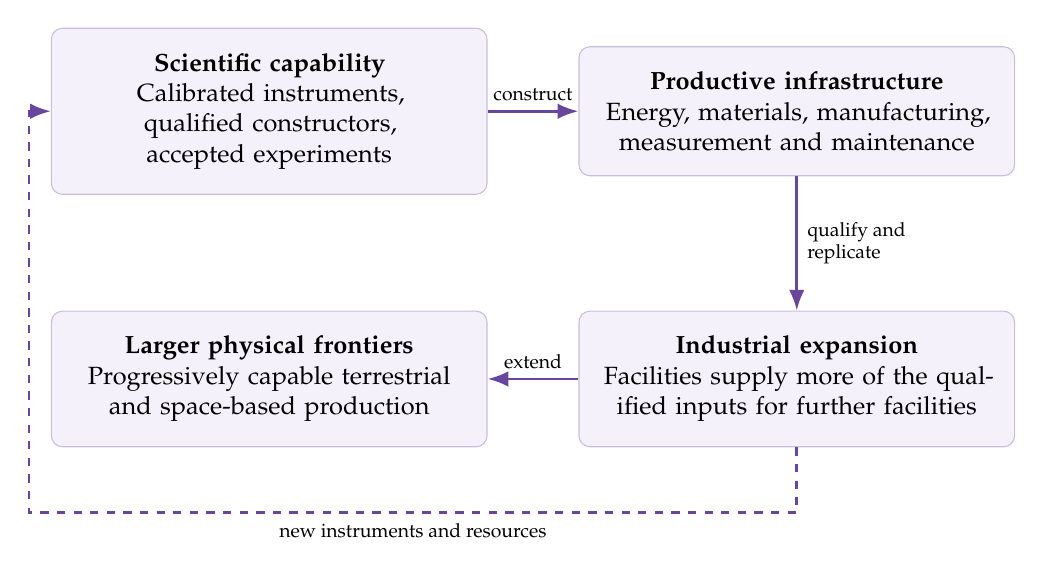
\begin{tikzpicture}[>=Latex,
box/.style={draw=violet!35,fill=pale,rounded corners=4pt,minimum height=1.5cm,text width=4.9cm,align=center,inner sep=9pt,font=\small},
flow/.style={->,line width=1pt,draw=violet}]
\node[box] (instruments) at (-3.35,2.1) {\textbf{Scientific capability}\\Calibrated instruments, qualified constructors, accepted experiments};
\node[box] (industry) at (3.35,2.1) {\textbf{Productive infrastructure}\\Energy, materials, manufacturing, measurement and maintenance};
\node[box] (closure) at (3.35,-1.3) {\textbf{Industrial expansion}\\Facilities supply more of the qualified inputs for further facilities};
\node[box] (horizon) at (-3.35,-1.3) {\textbf{Larger physical frontiers}\\Progressively capable terrestrial and space-based production};
\draw[flow] (instruments.east)--node[above,font=\scriptsize]{construct}(industry.west);
\draw[flow] (industry.south)--node[right,align=left,font=\scriptsize]{qualify and\\replicate}(closure.north);
\draw[flow] (closure.west)--node[above,font=\scriptsize]{extend}(horizon.east);
\draw[flow,dashed] (closure.south) -- (3.35,-3) -- node[below,font=\scriptsize]{new instruments and resources} (-6.4,-3) -- (-6.4,2.1) -- (instruments.west);
\end{tikzpicture}

\caption{A research pathway from qualified scientific instruments to larger productive systems. The feedback routes are part of the hypothesis. Each transition requires new acceptance, resources, commissioning and operating evidence; the diagram is not a forecast or an achieved deployment.}\label{fig:physical}
\end{figure}

At the first stage, the enterprise repeatedly delivers valuable scientific or engineering capabilities with complete costs and real buyer acceptance. At the second, it turns compatible capabilities into better instrumentation, energy systems, materials processes and manufacturing. At the third, those facilities supply a growing fraction of the qualified inputs needed for further capacity. Industrial self-expansion becomes a measured property of a production network, with remaining external dependencies visible.

The same constructive sequence applies at each stage. An instrument resolves a binding production uncertainty; an accepted process change supports a valuable service; collected returns and retained means support the next qualified installation. Equation~\eqref{eq:construction-gap} specifies the economic change required, Equation~\eqref{eq:capital} exposes the largest interim funding need, and Equation~\eqref{eq:renewal-window} tests the qualification date when its assumptions apply. The physical bottleneck determines whether the funded installation can actually increase useful output. This joins the commercial and industrial arguments through measurable dependencies.

NASA's 1982 study of advanced automation already proposed replicating lunar manufacturing concepts; such proposals are engineering antecedents, not evidence that industrial closure has been achieved \cite{nasa1982}.

At much later stages, analogous construction principles could apply to space-based energy and manufacturing. The relevant achievement would be an increasingly capable, reliable productive system using accessible resources and delivering human benefit at a much larger scale. Extrapolation to stellar scales is a horizon for research, not a numerical implication of the first profitable enterprise. Thermodynamics, orbital conditions, communications, material supply and lifecycle maintenance remain part of the problem.

\subsection{Sustainable advantage includes maintaining the world it depends on}
Long-run production requires reliable resources, acceptable consequences and continuing participation. Environmental damage, unmaintained assets, displaced costs and brittle dependencies can turn apparent profit into future loss or unacceptable harm. Count relevant lifecycle burdens in the actual project model and report physical outcomes alongside money. ``Sustainable'' here requires maintained technical service, financially viable renewal and acceptable resource use under the declared horizon; it is not an unlimited-growth guarantee.

This perspective also clarifies the social meaning of scale. Greater output is useful when it expands what people can choose and accomplish. Beneficiary value, producer surplus, available capital, qualified capacity and resource consumption should appear as separate measures. A large enterprise valuation does not measure a larger civilizational production frontier. Useful delivered capability does.

\section{The experiment that earns the next scale}
\subsection{Choose one consequential construction}
A campaign begins with a complete outcome and its current obstacle. Compare at least three materially different opportunity families when fresh selection is justified. Choose the candidate whose decisive test can most change a consequential construction or delivery decision. A large downstream consequence justifies serious research; it does not justify arbitrary confidence or a fabricated market value.

The selected experiment should state the proposed missing means, the strongest complete alternative and exactly what observation could change the verdict. Use established methods when appropriate. Blue Sky selection concerns the new attainable consequence of the complete arrangement; it does not require novelty in every component or an invented name for ordinary engineering.

\subsection{Freeze the comparison and resource treatment}
Before the decisive run, record task population, exposed development inputs, independent test inputs where available, outcome acceptance, rights, information access, timing, costs and failure handling. Include adaptive conventional construction, human-plus-AI and other autonomous providers as appropriate complete alternatives. The project's primary productivity comparison separately retains competent frontier AI/agents against competent 100\% human workers using conventional software; this comparison does not replace market outside options or the economic-enablement test.

Record actual internal human intervention and its full cost. A hybrid operation can be valuable and profitable while failing a strict autonomous-operation claim. Normal buyer consent and acceptance are distinct from labor inside the producer's operation; their real delay and friction still matter. Included model access does not make inference, tools or engineering economically free.

Each experiment has finite declared conditions, resources and stopping rules. Continue, repair, obtain an observation or retire the attempt based on its evidence. Finite experiments permit learning without imposing a universal business-size or mission-time ceiling. Preserve failed attempts and total search costs compactly; repeated selection after seeing outcomes cannot become an undisclosed search for a success.

\subsection{Jointly choose capital and the productive strategy}
Current project guidance treats starting capital and financing as decision variables for prospective work. US\$100,000 remains a reference comparison and the unchanged initial capital of historical frozen challenges. New studies must label their own capital, funding source, timing, fees, repayment, dilution and control assumptions. A larger capital scenario is an option to test, not an executed financing agreement or permission to spend.

Compare non-entry, staging, smaller and larger capital where relevant. Received capital belongs in the funding record; earnings belong in the profit record. Do not top up a historical account or remove its liabilities to obtain a preferred conclusion. A capital-intensive construction can be economically attractive yet inaccessible under the available financing menu; that is a concrete obstacle for the arrangement to solve.

\subsection{Measure the milestone on the right clock}
The program objective remains \textbf{US\$3 billion in trailing-365-day profit after complete modeled costs}. It is an unachieved milestone, not a maximum or a guarantee. Evaluate the declared native observer at a fixed preregistered endpoint after a complete operating horizon, with all applicable obligations and cost treatment disclosed. Preserve separately the profit definition used by that observer and any additional economic opportunity-cost adjustment.

Do not replace the measure with revenue, valuation, gross margin, cumulative multiyear earnings or annualized short-cohort arithmetic. Forecasts can guide a decision, but are labeled forecasts. Real commerce, native audited simulation and an authored analytical example each retain their own evidence status. A program can make useful technical progress while the milestone remains open.

\subsection{Require a consequential successor, then test the inventor}
After a qualified first outcome, choose a successor whose relevance follows from the construction. Record which means or available earnings it uses, what changes when they are removed, and whether the full successor is accepted and affordable. Give the strongest ordinary alternative the same resources and permission to reconstruct the means.

Only then investigate whether the process of finding such sequences has improved. Use fresh campaigns and the crossed policy/assets design. If ordinary reuse ties, retain the useful asset and narrow the method claim. If a simpler method wins, use it. If no complete arrangement pays, revise the outcome, market, means or contract rather than multiplying an uneconomic design.

\section{Conclusion}
SUPER ALPHA asks intelligence to do something economically consequential: construct valuable possibilities, build the means to deliver them, and sustain enough advantage to keep expanding productive power. The object of invention includes the scientific instrument, the production process, the evidence of acceptance and the voluntary arrangement that makes the activity worth doing.

The exact example identifies a constructive lever: change production and cooperation together so that a valuable activity acquires a viable surplus and price window. A failed window specifies how much must change. The largest interim cash deficit determines what capital the resulting sequence needs. Qualification time determines whether a funded successor arrives while its opportunity remains useful. These conditions connect invention to a sustainable succession of productive means. Strong ordinary alternatives, acceptance, causal successor benefit and useful physical output remain part of the evidence.

The long-range opportunity is an enterprise whose useful inventions improve the starting conditions for further useful inventions, whose accepted deliveries sustain that work, and whose qualified capabilities expand real production. Scientific capability foundries offer a concrete opening: construct a new instrument, establish the important activity it enables, and use the retained means to build a more consequential successor. Each earned advance can enlarge both the repertoire of useful actions and the questions worth asking next.

\thesis{Invent what becomes possible. Make its value sustain what comes next.}

\bigskip
\appendix
\section{Exact analytical specification}
\label{app:spec}
All numerical examples in Section~\ref{sec:example} are explicit authored constructions. They estimate no real price, demand, resource bill, financing offer or industrial yield. Costs use exact rational or integer arithmetic. The program generates complete rows, distinguishes counterfactual forced-delivery arithmetic from voluntary entry, and includes direct checks of the stated identities.

For cohort size $n$, fixed cost $F$, variable cost $c$, price $p$ and per-buyer value $v$, the cost functions are
\begin{equation}
C_{\rm individual}=n(F+c),\qquad C_{\rm pooled}=F+nc.
\end{equation}
For accepted voluntarily purchased delivery, revenue is $np$, profit is $np-C$, and buyer surplus is $n(v-p)$. The selected examples use $p<v$, so buyer acceptance does not rely on an indifference tie. At a ceiling price $v$, the profit expression is an upper bound; strict buyer participation requires $p<v$. For the original pooled method, $F=20,c=12,v=13$, hence even that upper bound is $n-20$. At $n=10$, it is negative. For the new method, $F=30,c=7$, the corresponding bound is $6n-30$ and the selected-price profit is $5n-30$.

The paired conditions show why a fixed cohort is part of the claim. For $n>20$, the old method can become viable at a suitable price strictly above 12 and below 13. At the selected price of 12 it loses 20 for every positive cohort size. A new method may move a cost threshold rather than create an activity that was physically impossible at every scale. Both can have significant value, but the evidence statement must preserve the workload and capital conditions.

The liquidity example uses actual starting equity of 100 to pay the complete model operating cost. Recognition of the unpaid 120 invoice produces period profit of 20, closing receivables of 120 and cash of zero. Collection changes cash and receivables, not profit again. A protected amount of 15 reduces cash available for new commitments without, by itself, becoming a second charge to profit.

The imitation case assumes an equivalent rival price cap of seven after construction. Its fixed capability is exogenous to that scenario. It is a counterexample to automatic capture, not a proved competitive equilibrium with identical entry costs. The successor commitment examples compare available cash with stated acquisition costs. Optional reconciliation scenarios stipulate successor receipts of 145 and 130, yielding complete-history cash of 155 and 135 and profit of 55 and 35. Those receipts are assumptions, with no empirical demand or profitability interpretation. The discovery matrix controls policy and asset contents separately and charges acquisition once per declared reuse horizon.

The ordered-capital examples use the 145-unit successor receipt and preserve total receipts of 265 and paid, expensed costs of 210. Changing collection order and holding 15 protected units changes the maximum interim deficit, while preserving conditional complete-history profit of 55. Capital of 100, 105 or 225 is a separately stated initial condition, never a top-up to an executed history. The renewal examples use arbitrary time units and a stipulated constant net settled surplus rate. The rate, qualification cost, qualification duration and opportunity deadline are model inputs; no timing or demand observation is implied.

\section{Reproduction and publication}
The source package includes the manuscript, bibliography, vector figures, exact analytical program, result snapshot, checks and citation metadata. Only public sources and original exposition are distributed.

From the source directory, use Python 3.11 or later for the analytical example:
\begin{lstlisting}
python3 companion.py --output /absolute/new/results.json
python3 -m unittest discover -s . -p 'test_companion.py' -v
\end{lstlisting}
With a standard TeX Live installation, Latin Modern, BibTeX, latexmk and Poppler:
\begin{lstlisting}
make check
python3 verify.py
python3 package.py --output /absolute/new/super-alpha-publication
\end{lstlisting}
The inspected PDF and source hashes are recorded in \texttt{PUBLICATION.json}. Rebuilds check normalized PDF text, references, page count and analytical results; PDF bytes can differ across TeX distributions. Release \texttt{super-alpha-v1.1.0} preserves this PDF, source ZIP and checksums; the original 1.0.0 release remains available. Edition 1.1 adds constructive economic targets, exact capital and renewal conditions, a fixed discovery denominator, corrected bibliographic attribution and clearer extracted-source instructions.

\textbf{Read and reproduce:} \href{https://montrealai.github.io/AGI-Alpha-Invention-Flywheel-Lab/super-alpha.html}{Browser reader and PDF} $\cdot$ \href{https://github.com/MontrealAI/AGI-Alpha-Invention-Flywheel-Lab/tree/main/docs/super-alpha}{Editable source and instructions}. Earlier editions and experimental histories remain available. Publication establishes inspectability, not unmeasured commercial or physical results.

\section{A compact record for the decisive experiment}
\begingroup\small
\begin{tabularx}{\linewidth}{@{}P{3.1cm}Y@{}}\toprule
Field & Required content\\\midrule
Consequence & The valuable complete outcome, beneficiary and why its current economic limitation matters.\\
Missing means & The specific observation, instrument, process, interface, agreement or complementary capability to construct.\\
Complete alternatives & Strong conventional construction, human and AI routes, self-service, rivals and no purchase; matched permissions and resources.\\
Acceptance & Frozen purpose, quality, deadline, rights and remaining obligations; independent reference or explicit uncertainty.\\
Resources and capital & Full search and delivery costs; actual or modeled capital provenance; timed funds, commitments and downside.\\
Capture & Buyer and supplier outside options, response to entry or imitation, service differentiation and renewal cost.\\
Successor & The new outcome, inherited means and funding source; an intervention testing the causal dependence.\\
Discovery & Fresh crossed policy/assets comparison if claiming a better invention process; otherwise keep the claim scoped.\\
Physical bridge & Measurements, qualification, useful output, material and energy inputs, commissioning and replication limits.\\
Decision & Accepted claim, failed condition, unresolved uncertainty and the next action that the result justifies.\\\bottomrule
\end{tabularx}\endgroup

\clearpage
\bibliographystyle{plainnat}
\bibliography{references}
\end{document}
